\documentclass[12pt]{article}
\usepackage{graphicx}
\usepackage [font=small, labelfont=bf]{caption}
\usepackage{listings}
\lstset{
basicstyle=\footnotesize\ttfamily,
numbers=left,
frame=bottomline,
framextopmargin=50pt,
}
\usepackage[colorlinks=true,pagebackref,linkcolor=blue]{hyperref}
\textwidth=7in
\textheight=9.5in
\topmargin=-1in
\headheight=0in
\headsep=.5in
\hoffset  -.85in

\lstset{
basicstyle=\footnotesize\ttfamily,
language=bash,
upquote=true,
breakatwhitespace=true,
columns=fullflexible,
keepspaces,
%numbers=none,
tabsize=3,
frame=blrt,
framextopmargin=5pt,
showstringspaces=false,
extendedchars=true
}

\pagestyle{empty}

\renewcommand{\thefootnote}{\fnsymbol{footnote}}

\begin{document}
Steven Su


\begin{center}
{\bf AMS 550.400 \quad HW SET 1\quad  Due Date:  Oct 10}\\
\vskip.2in
{\footnotesize Last Compiled on \today}
\end{center}

\setlength{\unitlength}{1in}

\begin{picture}(6,.1) 
\put(0,0) {\line(1,0){6.25}}         
\end{picture}

 

\renewcommand{\arraystretch}{2}

%\noindent\textbf{General Instruction:} 
%To complete the homework set, you are required to do the followings. 
%Your solutions must be typed in \LaTeX\ using the course homework
%template.  
%The progression of your homework solution is to be
%``recorded'' by making a git folder specifically for this homework
%set.  The burden of proof is on you, and if your git commit history
%is sparse, then you may be liable for a penalty.  
%A paper copy of the PDF output of your \LaTeX\ file is 
%to be submitted to your instructor in class on the due date.
%\emph{After} submitting the paper copy, but \emph{before} the end of
%the due date, you will upload your work to your github by making a remote repository
%specifically for the homework, and post the link to the repository 
%at the designated \emph{Discussion} forum in Blackboard by making 
%a thread just for you.  The repository name in your github should be
%\texttt{550400.homeworkset.1} and the discussion forum thread should
%be named \texttt{YourFirstNameMiddleInitialLastName}, e.g.,
%\texttt{BaracHObama} and \texttt{WillardMRommey}. 
%You have till the end of 
%the due date to finalize your github repository.  
%However, any commit made after the class time of the due date will be 
%inadmissible. \emph{Your attention to details in following this instruction will be 
%critical, and if not followed exactly at the time of collection, the
%homework set may be graded at $90\%$ of the full score}.

\vskip.25in
\noindent\textbf{Problem 1 (10 pts):}
%Assume that you are starting from ``scratch'' at the directory \verb+~/+.
%Provide a sequence of git/bash commands that yields a git folder with 
%a commit history such that:
%\begin{itemize}
%\item the \emph{master} branch has commits $A$, $B$, $C$, $X$ and $D$,
%\item the \emph{alt} branch has commits $A$, $B$, $X$,
%\end{itemize}
%Suppose that you are currently working on \texttt{master} branch. Draw 
%its commit history graph (i.e., the graph portion of the output of
%\verb+git log --graph --oneline+).  Next, assume that 
%you are on \texttt{alt} branch. Draw its commit history graph.\newline

\noindent To produce the two branches with the desired commit histories, the following GIT Bash commands can be executed:
\begin{lstlisting}
$ mkdir hondacivic.git
$ cd hondacivic.git
$ git init
$ vi main.txt #Create main.txt and add Line A
$ git add main.txt
$ git commit -m "A is Done"
$ vi main.txt #Add Line B to main.txt
$ git add .
$ git commit -m "B is Done"
$ git branch alt #Create branch named alt that has A and B commits
$ vi main.txt #Add Line C to main.txt
$ git add .
$ git commit -m "C is Done"
$ git checkout alt #Switch to alt branch
$ vi main.txt #Add Line X to main.txt in the alt branch
$ git add .
$ git commit -m "X is Done"
$ git checkout master #Switch to master branch
$ git merge alt #Merge the master branch with the alt branch
$ vi main.txt #Resolve the merge conflict
$ git add .
$ git commit -m "D is Done"
\end{lstlisting}  

\noindent The following figure represents the commit history graph when on the \texttt{master} branch:

\begin{figure}[h!]
\begin{center}
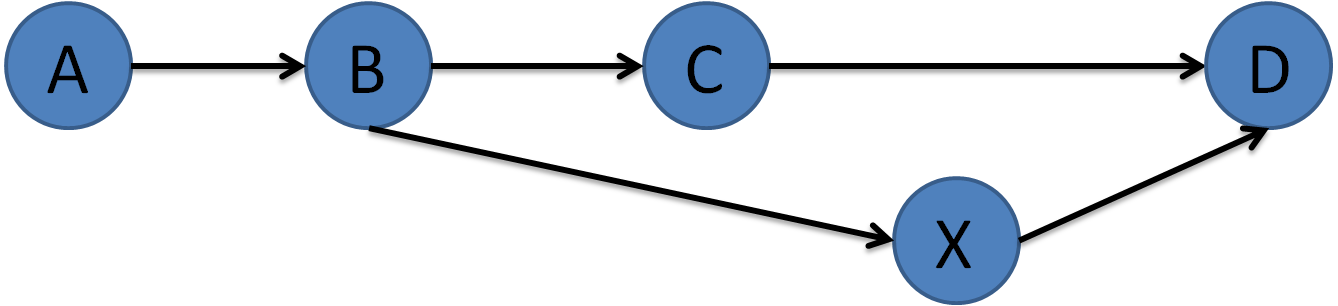
\includegraphics[width=3in]{Master.png}
\end{center}
\caption{The commit history graph when on the \texttt{master} branch}
\end{figure}

\noindent The following figure represents the commit history graph when on the \texttt{alt} branch:

\begin{figure}[h!]
\begin{center}
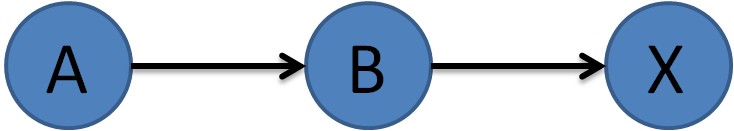
\includegraphics[width=3in]{Alt.png}
\end{center}
\caption{The commit history graph when on the \texttt{alt} branch}
\end{figure}

\newpage
%\vskip.25in
\noindent\textbf{Problem 2 (10 pts):}

\noindent Assume that you have created a new github repository at: 
\begin{center} 
\texttt{https://github.com/ssu7/PoemCollection.git}
\end{center} 
The following GIT Bash commands will produce what the problem asks for:
\begin{lstlisting}
$ git config --global user.name "Steven" #Sets the user name
$ git config --global user.email "stevenemail@yahoo.com" #Sets the email of the user
$ mkdir hondacrv.git #Makes new git folder
$ cd hondacrv.git #Changes the directory to the git folder
$ git init #Initializes the git folder
$ git remote add Stanza1 git://github.com/nhlee/550400.stanza1.git #Creates alias for stanza 1
$ git remote add Stanza2 git://github.com/nhlee/550400.stanza2.git #Creates alias for stanza 2
$ git remote add Stanza3 git://github.com/nhlee/550400.stanza3.git #Creates alias for stanza 3
$ git pull Stanza1 master
$ vi main.txt #Add Title to Poem in VIM
$ git add .
$ git commit -m "Stanza1 Added"
$ git pull Stanza2 master
$ vi main.txt # Resolve Merge Conflict in VIM
$ git add .
$ git commit -m "Stanza2 Added"
$ git pull Stanza3 master
$ vi main.txt # Resolve Merge Conflict in VIM
$ git add .
$ git commit -m "Stanza3 Added"
$ git remote add origin https://github.com/ssu7/PoemCollection.git
$ git push origin master #Pushes main.txt to the previously setup github repository
\end{lstlisting}


%Assume that you are starting from ``scratch'' at the directory \verb+~/+.
%Provide a sequence of git/bash commands that yields a git folder and 
%\begin{itemize}
%\item configure your git with your name and your email address,
%\item set up an alias for each of the git remotes listed below:
%\begin{verbatim}
%git://github.com/nhlee/550400.stanza1.git 
%git://github.com/nhlee/550400.stanza2.git 
%git://github.com/nhlee/550400.stanza3.git 
%\end{verbatim}
%Assume that each remote contains exactly single commit with 
%a txt file for a single (different) stanza,
%\item pull to combine three stanzas of a poem,
%\item after the first pull, add the title of the poem,
%\item after the second and third pull, resolve the merge conflict,
%\item after resolving the third pull merge conflict, push the result
%  to your (newly created) remote repository. 
%\end{itemize}

\newpage
\noindent\textbf{Problem 3 (40 pts):}

\paragraph{} The issue of asynchronous collaboration on a class project is a common problem faced by many college students. Git, a free and open source version control software, offers a possible solution to this issue. In the proposed situation, there are 4 students, A, B, C, and D, who will all be working on different portions of a LaTeX/Beamer presentation. The main problem in this situation is to model a GIT workflow process that minimizes the amount of merge conflict that need to be resolved. 

\paragraph{} As stated in the problem statement, we will assume that each student will only edit the section of the Beamer presenation in \texttt{main.txt} which they are responsible for, and will NOT edit any other sections. Furthermore, as previously stated in the problem statement, none of the sections in \texttt{main.txt} overlap. In addition, if a student's section requires additional LaTeX packages, that student will add the necessary packages to the preamble portion of \texttt{main.txt}. Under these assumptions, the preamble part of \texttt{main.txt} is an exogenous variable. The endogenous variables (i.e. what we are interested in studying) are how effective different git workflows are at minimizing merge conflict resolutions. More specifically the endogenous variables can be thought of as how changes and edits to the the different sections of the Beamer presentation (\emph{Introduction}, \emph{Problem Statement}, \emph{Timeline}, and \emph{Deliverables}) are comitted using git. The endogenous and exogenous variables are interrelated in that the workflow for committing changes to \texttt{main.txt} (i.e the endogenous variable) will affect how often and how smoothly the preamble portion of \texttt{main.txt} is merged (i.e. the exogenous variable). In addition, we will further assume that all students are proficient at using git, and as such, the git proficiency of the students is an unimportant and ignored variable.

\paragraph{} One possible workflow process that could be employed in this situation uses a remote git repository with a \texttt{master} branch and 4 other branches, say \texttt{A}, \texttt{B}, \texttt{C}, and \texttt{D}, one for each student. In this workflow, each student will clone the remote git repository onto their computer and (i.e. create a local git repository). Each student will then edit/create their respective section of \texttt{main.txt} while commiting these changes to only their assigned branch in their local repository. After a student is satisfied with his/her section of \texttt{main.txt}, he/she can then merge his/her final local branch to his/her local \texttt{master} branch. After this, the student will push both his/her local assigned branch to the corresponding remote assigned branch as well as his/her local \texttt{master} branch to the remote \texttt{master} branch. After a student pushes his/her local \texttt{master} branch to the remote \texttt{master} branch, he/she will be responsible for merging their section into the existing file. Since each student only edits his/her respective section of \texttt{main.txt}, the merge process should be fairly straight-forward and easy. Each section of \texttt{main.txt} in the \texttt{master} branch of the remote repository should be empty up until the student who is responsible for that section pushes his/her version of the presentation to the \texttt{master} branch in the remote repository. A student will only need to check to see if his/her section has been added correctly, and that the other sections haven't been affected (which they shouldn't). The only portion of \texttt{main.txt} that this is not true of is the preamble portion in which case a merge conflict may arise. However merging this section should be easy as well; each student should keep what is in the preamble of the version in the remote repository and add in the changes they made. 

\paragraph{}Using this workflow, the \texttt{master} branch in the remote repository should be very clean: the only nodes that appear in the commit history should be when each student adds his/her finalized section of the presentation. This workflow also allows for the edits and commits made by each student for their section of the presentation to be remembered through the commit history of the 4 student branches. This workflow also minimizes the number of merges that need to be made since each student will only merge their contributions to the remote \texttt{master} branch once.

\paragraph{} Another possible workflow process uses one remote group repository with a single \texttt{master} branch. Each student will again clone the remote repository onto their own computer and create a local repository. However in this workflow, each student will edit and commit changes directly to his/her local \texttt{master} branch and every so often push and merge these commits to the remote \texttt{master} branch. Students will continue doing this until they are all satisfied with their sections. At the end of all the commits, the final, completed version of \texttt{main.txt} will be in the final commit of the remote \texttt{master} branch. 

\paragraph{} This workflow involves more pushes and merges to the remote \texttt{master} branch then necessary. Most of these merges should still be straight-forward since each student will only make changes to their own section of \texttt{main.txt} which does not overlap with any other section. However merges that involve the preamble portion will again require special attention since all 4 students can potentially change this portion of the LaTeX file. This workflow also mixes the commit histories of each section into the remote \texttt{master} branch's commit history which could potentially become very messy. This workflow also fails to utilize branching, which is a main feature of git.

\paragraph{} There is a causal relationship between the number of times merges occur and the number of merge conflicts: the greater the number of merges, the greater the possible number of merge conflicts. The mechanism by which this causal relationship happens can be easily understood: anytime a merge happens, there is a chance that a merge conflict will arise which then needs to be resolved. This causal relationship is strong and consistent in its association. The causal relationship is also temporal in its nature: the cause (merges) precedes the effect (merge conflicts). Therefore by mimimizing the total times the students merge files, the first proposed workflow in essence minimizes the potential number of merge conflicts that need to be resolved. As such, the first proposed workflow model solves the previously formulated problem which was to develop a workflow strategy which minimizes merge conflict resolutions, and is thus a useful workflow model. We therefore can recommend using the first proposed workflow over the second.

\paragraph{} We can test the recommended workflow model to see if it is indeed better then the second workflow by  having 4 students working on a group presentation employ the recommended workflow scheme and having another group of 4 students use the second workflow scheme. Whichever group of students encounters less merge conflicts and has less trouble with merge conflict resolutions is the group that used the better workflow. In theory, the group using the recommended workflow should only have 4 merge conflicts to resolve in a worst case scenario. (Each student will only push their finalized version of their section to the remote \texttt{master} branch once.) The other group could potentially have far more merge conflicts since they are continually pushing and merging their unfinished work to the same remote \texttt{master} branch. Thus by using logic we can conclude that our recommended workflow does indeed minimize merge conflicts and is better than the other proposed workflow. 

%Consider a team of four students, say, $A$, $B$, $C$ and $D$, 
%who just started working 
%on writing a \texttt{latex/beamer} file, say \texttt{main.tex}, 
%for a class presentation of their work statement.  
%Assume that they do not wish to coordinate their schedules for a
%concurrent group meeting (both virtually and physically).  
%Assume that:
%\begin{itemize}
%\item $A$ is in charge of \emph{Introduction},
%\item $B$ is of \emph{Problem Statement}, 
%\item $C$ is of  \emph{Timeline},
%\item $D$ is of \emph{Deliverable} part of the presentation.  
%\end{itemize}
%In other words, their contributions to \texttt{main.tex} do not overlap.
%Then, 
%\begin{itemize}
%\item first, devise a work flow strategy for the team so that they can
%  collaborate asynchronously using \texttt{git},
%\item next, devise yet another \texttt{git} strategy different from your earlier
%  proposal.  
%\end{itemize}
%Finally,
%\begin{itemize}
%\item discuss the strength and weakness of each of your proposed strategies in terms of merge
%conflicts resolution,
%\item make the final recommendation.  
%\end{itemize}
%In order to answer this question, \emph{build}
%a mathematical model, \emph{following} the guideline from IMM. 
%Use Section 1.4 and Section 1.5 of IMM as \emph{role models}.    
%For example, you are to identify which variables  are exogenous 
%and which are endogenous.  More specifically, among other things, 
%in your model, is the preamble part of \texttt{main.tex} an endogenous 
%or exogenous variable?  
%Note also that in addition to this issue, there are other issues that
%you are to consider.  So, \emph{be sure to consult IMM}. 
\vskip0.25in
\newpage
\noindent\textbf{Problem 4 (aka.\ Fair Play, 40 pts):}

\paragraph{} Tennis is an exciting sport to watch once a person understands its rules. In a tennis match, one player, say Player A, starts out as a server and the other player, say Player B, starts as the reciever. The winner of a \emph{game} is the first player to 4 points. The players switch serve after each \emph{game}. The first player to win 6 out of 11 \emph{games} wins the \emph{set}. Note that a player must win by 2 \emph{games} to win a \emph{set}, so more then 11 \emph{games} could be played per \emph{set}. The first player to win 3 out of 5 \emph{sets} wins the entire \emph{match}.

\paragraph{} The question we are trying to answer is whether serving first gives an advantage to a player. This is the same as asking whether the player who serves first is more likely to win the match then the other player who recieves first. In order to simplify the model, we will neglect any innate skill difference between the two players and assume that each player is of equal skill as the other player. In other words, we will assume that the probability of Player A winning a game when Player A is serving is equal to the probabiity that Player B will win a game when Player B is serving. Let us denote this probability as $P_{game}$.

\paragraph{} By making this assumption, we are making the players' skill difference a unimportant variable and ignoring it. Another unimportant variable that we will ignore is any and all psychological factors that may impact players when they are competing. The exogenous variable in this problem is the probability of a player winning a game when he is serving, which as previously stated, is $P_{game}$ for both players. The endogenous variable is the probability that a player wins the match; let us denote this $P_{matchA}$ for Player A and $P_{matchB}$ for Player B.

\paragraph{} To simplify our model, we will consider an abbreviated tennis match and analyze the match at the \emph{games} level. Suppose that the first player to win 2 games wins a set, and that the first player to win 1 set wins the match. For now we will ignore the ``win by 2 games rule.'' Imagine that each game is a Bernouli trial (i.e. a coinflip): the serving player has $P_{game}$ chance of winning and $1-P_{game}$ chance of losing. Note that this means that games are independent of one another. Suppose Player A serves the first game. He has $P_{game}$ chance of winning that match, while Player B (the reciever) has $1-P_{game}$ chance of winning the game. In the next game Player B serves and Player A receives, and thus, Player B now has $P_{game}$ chance of winning the second game and Player A now has $1-P_{game}$ chance of winning the second game. The probabilities once again switch for the third game and so on.

\paragraph{}Note that the set (and thus the match) could end after 2 games} or all 3 games could be needed to decide the winner of the set. Thus we have the following equations:

\begin{equation}
P_{matchA}=P_{game}(1-P_{game})+P_{game}(P_{game})P_{game}+(1-P_{game})(1-P_{game})P_{game}
\label{1}
\end{equation}
\begin{equation}
P_{matchB}=(1-P_{game})P_{game}+(1-P_{game})(1-P_{game})(1-P_{game})+P_{game}(P_{game})(1-P_{game})
\label{2}
\end{equation}
The first product term in (\ref{1}) represents the probability of Player A winning the set by winning the first 2 games. The second product term in (\ref{1}) represents the probability of Player A winning the first game, losing the second, and winning the third. The third term in (\ref{1}) represents the probability of Player A losing the first game and winning the second and third games. Similarily the first product term in (\ref{2}) represents the probability of Player B winning the first 2 games. The second term in (\ref{2}) represents the probability of Player B winning the first game, losing the second game, and winning the third game. The last term in (\ref{2}) represents the probability of Player B losing the first game and winning the second and third games. Careful analysis of (\ref{1}) and (\ref{2}) shows that if $P_{game}>0.5$ then $P_{matchA}>P_{matchB}$, and serving first is advantageous. If $P_{game}<0.5$, then $P_{matchA}<P_{matchB}$, and  serving first is disadvantageous. Note that if $P_{game}=0.5$, then $P_{matchA}=P_{matchB}$, and we find that serving first does not affect the fairness of tennis.  

\paragraph{} In the prevous analysis we ignored the ``win by 2 games rule''; we now add it to our analysis. By adding this rule into our model, we can now see just how important the ``win by 2 games rule'' truly is. A set (and thus the match) can ONLY be decided when a player has won 2 games in a row. Note that if a player is down one game to his opponent, he can win the set by winning 3 games in a row. However, winning 3 games in a row entails winning 2 games in a row. (i.e. winning 1 game and then winning the next 2 games in a row.) Note that when a player is up by 1 game, he is in the process of winning 2 games in a row; he has won the previous game and just needs to win the upcoming game. This logic shows that it is not necessary to consider situations where one player is ahead by 1 game. Being ahead by 1 game simply means that a player is in the process of trying to win 2 games in a row. As such, we will only consider situations where the two players are tied in games.

\paragraph{} Note that the probability of Player A winning 2 games in a row is equal to the probability of Player B winning 2 games in a row:
\begin{equation}
P_{Win\ 2\ Consecutive\ Games,\ Player\ A}=P_{game}(1-P_{game})=P_{Win\ 2\ Consecutive\ Games,\ Player\ B}
\label{eq:3}
\end{equation}
Because serving alternates between games, we can see that (\ref{eq:3}) is memoryless: regardless of how many games have been played in the past, the probability of winning the next 2 games in a row is always $P_{game}(1-P_{game})$ for either player. A player must always serve one game and recieve the other. Consider the simple case when we are just starting a match and 0 games have been played. The probabilty of A winning the first two games and thus the set and match is $P_{game}(1-P_{game})$. The probability of B winning the first two games (and thus the set and match) is also $P_{game}(1-P_{game})$. Taking this to the extreme, when the players are tied 1001 games to 1001 games, each player still has a $P_{game}(1-P_{game})$ probability of winning the next two games and thus the set and match.
 
\paragraph{} Based on (\ref{eq:3}) and our analysis above we can see that when the ``win by 2 games rule'' is in place, for all $P_{game} \in (0,1)$, $P_{matchA}=P_{matchB}$, and thus serving first gives no advantage to a player. This result is different from our previous analysis when we ignored the ``win by 2 rule'', which concluded that if $P_{game}>0.5$, then serving first is advantageous, and if $P_{game}<0.5$, then then serving first is disadvantageous. When ignoring the ``win by 2 rule'', the only time serving first is not advantageous or disadvantageous is when $P_{game}=0.5$. We see that the ``win by 2 rule'' makes it so that serving first offers no advantage or disadvantage to a player.

%Note that the win by 2 games rule only applies if 3 games have been previously played. There are only 2 situations to consider: either Player A is ahead 2 games to 1 or Player B is ahead 2 games to 1.
%\paragraph{} First consider the situation where Player A is ahead 2 games to 1. We see that regardless of how Player A came to be ahead 2 games to 1 (either he won games 1 and 3 or won games 2 and 3), the probability of him winning the next game and thus the set is $(1-P_{game})$. Now consider the situation where Player B is ahead 2 games to 1. We see that regardless of how Player B came to the 2 games to 1 lead (either he won games 1 and 3 or won games 2 and 3), the probability of him winning the next game and thus the set is $P_{game}$. Thus incorporating this element into (\ref{1}) and (\ref{2}) we get:
%\begin{equation}
%P_{matchA}=P_{game}(1-P_{game})+[P_{game}(P_{game})P_{game}+(1-P_{game})(1-P_{game})P_{game}](1-P_{game})
%\label{3}
%\end{equation} 
%\begin{equation}
%P_{matchB}=(1-P_{game})P_{game}+[(1-P_{game})(1-P_{game})(1-P_{game})+P_{game}(P_{game})(1-P_{game})]P_{game}
%\label{4}
%\end{equation}
%
%\paragraph{} The first terms in (\ref{3}) and (\ref{4}) represent the same thing as they did in (\ref{1}) and (\ref{2}), respectively. The second term in (\ref{3}) is the probability of Player A being up 2 games to 1 game and then winning the 4th game and thus the set and match. Similarily, the second term in (\ref{4}) is the probability of Player B being up 2 games to 1 game and then winning the 4th game and thus the set and match. 
%
%\paragraph{}Careful algebraic analysis of (\ref{3}) and (\ref{4}) show that they are equal to each other, meaning that $P_{matchA}=P_{matchB}$ for all $P_{game}\in(0,1)$. Thus we conclude that serving first in a tennis match does not provide an advantage to a player. Note that the 3 only model up to 4 games since that is all that is necessary. Player A being up 3 to 2 or 4 to 3 or even 100 to 99 games is similar to the situation where he is up 2 to 1 games. The same is also true for Player B. The equations to model these situations would just have more terms in them, but mathematically and logically, they follow (\ref{3}) and (\ref{4}).

\paragraph{} The model of fairness we outlined above is useful if we can find an empirical value of $P_{game}$. We can find this value by obtaining a large data set of professional tennis match statistics. $P_{game}$ will be equal to the fraction of games that professional players win when they are serving, averaged for all players. After coming up with this value for $P_{game}$, we can input it into (\ref{eq:3}) and get a value for $P_{game}(1-P_{game})$. We can then compare this predicted value to the data set value (i.e the fraction of the time that 2 games are won in a row). We can also use the actual data to see if our prediction that serving first is neither advantageous or disadvantageous is true by computing the percentage of actual matches that are won by the player who serves first. 

%(i.e the fraction of the time a player wins two games in a row)

%Answer the following question:
%\begin{verse}
%Is the tennis game fair?
%\end{verse}
%Note that unlike Problem 3, this question is vaguely stated.
%This is intensional, whence to begin, you will first need to clarify
%what exactly your question is.
%You may use the class discussion on this particular 
%problem, but you \emph{may not} directly refer to our 
%discussion.  Instead, formulate the model carefully but concisely in 
%your own words.   

%\vskip0.25in
%\noindent\textbf{Final Remarks about Problem 3 \& Problem 4:} 
%They are open-ended problems.  However, your scores will be determined
%by how well do you follow the exposition style outlined by IMM and
%WMA.  For both problems, your write-up should be 
%\begin{itemize}
%\item self-contained,
%\item covering all four parts of Section 1.3 of IMM,
%\item paying a particular attention to any causal relation that you
%  might be investigating, following Chapter 3 of WMA,
%\item answering questions that are explicitly asked in the problem statements.
%\end{itemize}
%For Problem 3, focus mostly on Step 2 and Step 3 of Section
%1.3 of IMM.  For Problem 4, focus mostly on Step 1 and Step
%2.  For each problem, minimum 1 pages and maximum 2 pages.
\end{document}
